\chapter{Ergebnisse}
\label{sec:ergebnisse}

\section{Grafiken und Text}

Im Ergebnis-Teil sollen die Ergebnisse vorgestellt werden, für das Beispiel einer Software-Entwicklung also die mit der entwickelten Software erzielbaren 
Ergebnisse. Im Falle einer Simulationsentwicklung könnte man hier verschiedene Simulationsszenarien definieren und unter verschiedenen Randbedingungen 
vorstellen.

Es ist dabei darauf zu achten, dass ein ausgewogenes Verhältnis von Bild und Text besteht. Alle in den Plots vorkommenden Linien sind zu erklären. Jeder Plot 
benötigt eine vollständige Achsenbeschriftung und ggf. eine Legende. Eine Grafik muss immer selbsterklärend sein, d.h. man muss mit Grafik und Bildunterschrift 
allein in der Lage sein, das Gezeigte zu verstehen.

Auch bei den Ergebnissen soll weiterhin auf den roten Faden geachtet werden. Der Leser soll Stärken und Schwächen des Tools / der Simulation / der Konstruktion 
kennenlernen.

Um Plots zu erstellen, lässt sich ebenfalls TikZ nutzen (wie auch für WBS, Zeitplan, etc.). Der Vorteil ist, dass alle Beschriftungen einer Grafik auch 
dieselbe Schrift und -größe tragen, wie auch der Haupttext. Darüber hinaus sind TikZ-Grafiken auch Vektorgrafiken, sodass Qualitätsverluste nicht zu erwarten 
sind, wie das etwa bei PNG oder JPG der Fall wäre.

Beispiel für das Plotten von zwei verschiedenen Kurven aus Datenfiles, welches das Paket \tb{pgfplots} nutzt (siehe auch sehr ausführliche Dokumentation mit 
zahlreichen Beispielen online!):

\begin{figure}[h!]
 \centering
 \begin{tikzpicture}
  \begin{axis}[
       xlabel = {Anzahl entfernter Objekte pro Mission},
       ylabel = {Missionskosten in USD/kg (FY14)},
       xmin   = 2,
       xmax   = 10,
       xtick  = {2,4,6,8,10},
       minor x tick num={1},
       minor y tick num={1},
       %ymin   = 0,
       %ymax   = 400000,
       scaled ticks = true,
       ymajorgrids,
       yminorgrids,
       xmajorgrids,
       xminorgrids,
       legend entries={$m_t=5.5\;t$, $m_t=1.4\;t$},
       legend style={at={(0.5,-0.2)}, anchor=north, draw=none},
       legend cell align = left
  ]
    \addplot[mark=square,   mark options=solid, solid]              	table {tikz/data/mtm-cost-per-kg-cp.dat};
    \addplot[mark=asterisk, mark options=solid, densely dashed]     	table {tikz/data/mtm-cost-per-kg-cp-low-mass.dat};    
  
  \end{axis}
\end{tikzpicture}
 \caption{Vergleich der Kosten pro kg entfernten Schrotts für hohe und mittlere Objektmassen.\label{abb:vergleich}}
\end{figure}

Auch das Plotten von Funktionen ist sehr einfach, wie \abb{abb:x2} für das simple Beispiel einer quadratischen Funktion zeigt.

\begin{figure}[h!]
  \centering
  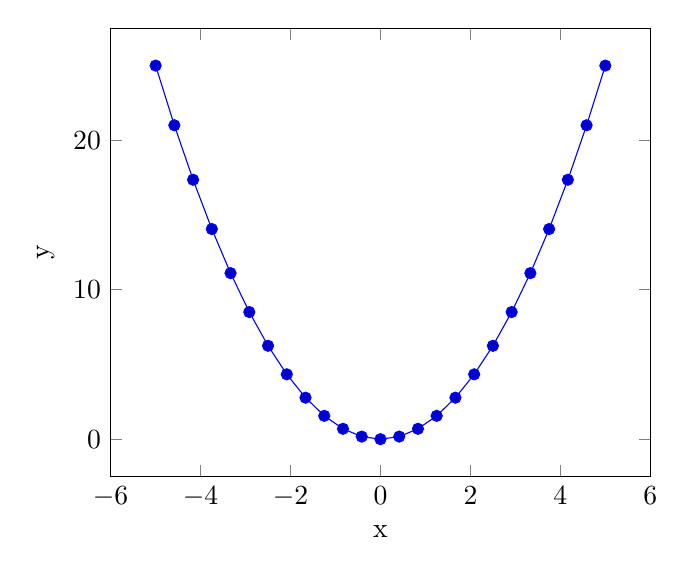
\begin{tikzpicture}
    \begin{axis}[
       xlabel = x,
       ylabel = y
    ]
    
      \addplot {x^2};
  
    \end{axis}
  \end{tikzpicture}
  \caption{Die Funktion $y=x^2$.\label{abb:x2}}
\end{figure}

Sollte nicht TikZ verwendet werden, ist auch \tb{Gnuplot} zu empfehlen. Allerdings ist dann darauf zu achten, dass sämtliche Beschriftungen gut lesbar sind und 
auch die Grafiken in der entsprechenden Auflösung, ohne Artefakte, etc. im Dokument erscheinen.

\section{Erstellen dieses Dokuments}

Um das vorliegende Dokument zu erstellen, muss die Datei \ts{vorlage.tex} mit \tb{pdflatex} kompiliert werden. Alle üblichen Entwicklungsumgebungen für Latex 
stellen diese Funktion zur Verfügung (z.B. Kile unter Linux, MikTeX unter Windows, oder TeXShop auf dem Mac).

Dazu wird die Dokumentenklasse \tb{tubsreprt} benötigt, welche das Corporate Design der TU Braunschweig umsetzt. Diese findet man, samt Installationsanleitung 
unter \url{http://www.enricojoerns.de/tubslatex/} (aktueller Release: 1.0.3).

Wichtig, damit auch das Symbol- und Abkürzungverzeichnis funktionieren, ist die Ausführung des Befehls \tb{makeglossaries} ebenfalls auf die Datei 
\ts{vorlage.tex} angewandt. Die Erstellung des Dokuments verläuft also in mehreren Schritten:
\begin{itemize}
 \item pdflatex auf \ts{vorlage.tex} (erzeugt die für makeglossaries benötigten Dateien!)
 \item makeglossaries auf \ts{vorlage.tex} (erstellt das Abkürzungs- und Symbolverzeichnis)
 \item pdflatex auf \ts{vorlage.tex} (ggf. mehrmals!) erstellt nun das Dokument mit allen Referenzen
\end{itemize}
Der Befehl makeglossaries muss in der Regel manuell in der Entwicklungsumgebung eingestellt werden, was für die verschiedenen Typen unterschiedlich ist. Daher 
am besten Google befragen (z.B. ``Kile makeglossaries'').